% !TeX encoding = UTF-8
\documentclass[a4paper, 11pt]{article}

% packages
\usepackage[czech]{babel}
\usepackage[utf8]{inputenc}
\usepackage[left=2cm, text={17cm, 24cm}, top=3cm]{geometry}
\usepackage[IL2]{fontenc}
\usepackage{bookman}
\usepackage[numbers]{natbib}
\usepackage[hidelinks]{hyperref}
\usepackage{graphicx}
\usepackage{picture}

\bibliographystyle{czplain}

\renewcommand{\bibsection}{\section{\bibname}}

\graphicspath{ {./img/} }

\begin{document}

\begin{titlepage}
\begin{center}

\textsc{{\Huge Vysoké učení technické v~Brně}\\\medskip{\huge Fakulta informačních technologií}}

\vspace{\stretch{0.390}} 

% -----

{\LARGE Mikroprocesorové a vestavěné systémy}
\medskip

{\Huge Demonstrace využití rozhraní USB}

% -----

\vspace{\stretch{0.610}}

{\Large \today \hfill Jakub Frýz}

\end{center}
\end{titlepage}

\tableofcontents
\pagebreak

\section{Úvod}

\subsection{Zadání}

S využitím nezbytných prostředků jazyka C, knihoven dostupných na webu společnosti Freescale a vývojových nástrojů vytvořte jednoduchou demonstrační aplikaci pro ARM na FITkitu3, která bude vhodným způsobem ilustrovat možnosti využití rozhraní USB. Vytvořte prezentaci v ppt+pdf s názornými ukázkami tvorby aplikace tak, aby byla srozumitelná pro studenty BP a případně použitelná pro výukové účely.

\subsection{Použité SDK}

Projekt byl sestaven pomocí MCUXpresso SDK pro KDS.

\pagebreak

\section{Projekt}

Projekt je upravený příklad pro \textbf{SD kartu} z balíčku příkladů SDK.

\subsection{Spuštění}

K provozu projektu je potřeba do FitKitu vložit SD kartu. Následně po připojení FitKitu do~USB portu pomocí kabelu je operačním systémem rozpoznán jako USB flash disk.

\subsection{Popis}

\subsubsection{Důležité funkce}

Nejdůležitější fce projektu jsou \texttt{USB\_DeviceCallback()} a \texttt{USB\_DeviceMscCallback()}. Tyto funkce se spouštějí při přerušení.

Funkce \texttt{USB\_DeviceCallback()} obsluhuje klasické události pro USB  jako je např. získání jednotlivých popisovačů a funkce \texttt{USB\_DeviceMscCallback()} zase obsluhuje události specifické pro zařízení třídy typu disk jako je např. žádost a odpověď pro čtení a zápis.

\subsubsection{Popisovače}

Všechny USB zařízení obsahují hierarchii popisovačů, které popisují hostiteli různé informace jako typ zařízení, výrobce, podporovaná verze USB, počet koncových bodů, atd.

\begin{center}
	\medskip
	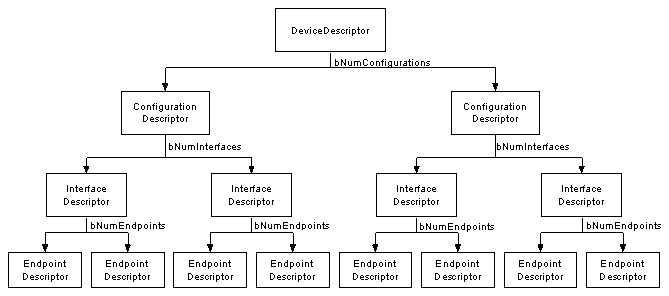
\includegraphics[width=0.9\textwidth]{desctree}
	\medskip
\end{center}

Popisovače jsou v souborech \texttt{usb\_device\_descriptor.c} \& \texttt{usb\_device\_descriptor.h}.
Najdeme zde jeden popisovač zařízení (\texttt{DeviceDescriptor}), jeden popisovač konfigurace (\texttt{ConfigurationDesriptor}), jeden popisovač rozhraní (\texttt{InterfaceDescriptor}), dva popisovače koncových bodů (\texttt{EndPointDescriptor}) a pět textových popisovačů \linebreak (\texttt{StringDescriptor}).

Každý z těchto popisovačů má daný formát, co má obsahovat. Aby zařízení bylo rozpoznáno jako uložiště, musí mít popisovač zařízení nastavenou třídu na \texttt{0} a popisovač rozhraní musí mít třídu nastavenou na \texttt{8}. Nultý textový popisovač by měl obsahovat seznam podporovaných jazyků (\texttt{0x0409} = Angličtina - USA, \texttt{0x09} = Angličtina, \texttt{0x04} = Čínština). Popisovače koncových bodů se používají pro popis všech koncových bodů kromě nultého. Dále jsou v popisovačích uloženy informace jako ID~výrobce, ID~produktu, sériové číslo, atd. Některé z těchto atributů jsou přiřazeny organizací USB.


\subsection{Omezení}

\begin{itemize}
	\item velikost bufferů pro zápis a čtení je nastavena na 1024 bitů, což má za následek pomalý přenos u větších souborů \\ \textbf{ŘEŠENÍ:} navýšení těchto hodnot v souboru \texttt{disk\_sdcard.h} makra \linebreak \texttt{USB\_DEVICE\_MSC\_WRITE\_BUFF\_SIZE} \& \texttt{USB\_DEVICE\_MSC\_READ\_BUFF\_SIZE}
\end{itemize}



\pagebreak
\begin{flushleft}
\nocite{*}
\bibliography{dokumentace}
\end{flushleft}

\end{document}
